\subsection{Hyperbolische PDGL}
\begin{minipage}{14cm}
	PDGL: $\partFrac{^2u}{t^2}-a^2\partFrac{^2 u}{x^2}=0\qquad \Omega=\left\{(x,t)|t>0\right\}\qquad u_0=u(x_0,0)$\\
	
	Trick: $(\partial_t +a\partial_x)(\partial_t-a\partial_x)u=(\partial_t^2-a^2\partial_x^2)u=0$\qquad(f�r konstante Geschwindigkeit $a$)\\
	
	Zwei m�gliche L�sungen: $\underset{\text{\cfbox{red}{Nach rechts laufende Welle}}}{\underbrace{(\partial_t +a\partial_x)u=0}}\qquad \underset{\text{\cfbox{black}{Nach links laufende Welle}}}{\underbrace{(\partial_t-a\partial_x)u=0}}$\\
	
	L�sung mittels Charakteristiken: $\partFrac{}{s}
	\begin{Bmatrix}
		x(s)\\
		t(s)\\
		u(s)
	\end{Bmatrix}=
	\begin{Bmatrix}
		\pm a\\
		1\\
		0
	\end{Bmatrix}
	\begin{array}{ll}
		\Rightarrow&x=\pm as +x_0\\
		\Rightarrow&t= s +t_0=s\qquad (t_0=0)\\
		\Rightarrow&u=u_0\\
	\end{array}
	$\\
	
	$x=\pm at+x_0\quad\Rightarrow\quad x_0=x\mp at\quad\Rightarrow\quad u(x,t)=u_0(x\mp at)$\\
	
	Allgemeine L�sung aus Linearkombination: $\boxed{u(x,t)=u_+(x+at)+u_-(x-at)}$\\
	
	$\Rightarrow$ Es werden \textbf{zwei} Anfangsbedingungen ben�tigt um $u_+$ \textbf{und} $u_-$ zu bestimmen.\\
	
	z.B.: $u(x,0)=u_0(x)\qquad \partFrac{u}{t}(x,0)=g_0(x)$
	\end{minipage}
	\hfill
	\begin{minipage}{5cm}
	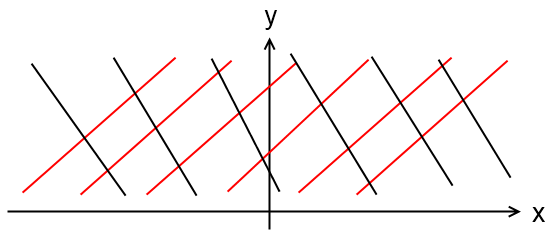
\includegraphics[width=5cm]{Content/Theory/linksRechts}
	\end{minipage}